\hypertarget{XMLManual_XMLTOC}{}\subsection{Table Of Contents}\label{XMLManual_XMLTOC}

\begin{DoxyItemize}
\item \hyperlink{XMLManual_XMLOverview}{Overview}
\begin{DoxyItemize}
\item \hyperlink{XMLManual_XMLIntroduction}{Introduction}
\item \hyperlink{XMLManual_XMLFeedBack}{FeedBack}
\item \hyperlink{XMLManual_XMLAcknowledgments}{Acknowledgments}
\item \hyperlink{XMLManual_XMLLicense}{License}
\end{DoxyItemize}
\item \hyperlink{XMLManual_XMLDOM}{Document Object Model}
\item \hyperlink{XMLManual_XMLLoading}{Loading Documents}
\item \hyperlink{XMLManual_XMLAccessing}{Accessing Document Data}
\item \hyperlink{XMLManual_XMLModifying}{Modifiying Document}
\item \hyperlink{XMLManual_XMLSaving}{Saving Documents}
\item \hyperlink{XMLManual_XMLXPath}{XMLXPath} \par
 \par
 
\end{DoxyItemize}\hypertarget{XMLManual_XMLOverview}{}\subsection{Overview}\label{XMLManual_XMLOverview}

\begin{DoxyItemize}
\item \hyperlink{XMLManual_XMLIntroduction}{Introduction}
\item \hyperlink{XMLManual_XMLFeedBack}{FeedBack}
\item \hyperlink{XMLManual_XMLAcknowledgments}{Acknowledgments}
\item \hyperlink{XMLManual_XMLLicense}{License}
\end{DoxyItemize}\hypertarget{XMLManual_XMLIntroduction}{}\subsubsection{Introduction}\label{XMLManual_XMLIntroduction}
\hyperlink{namespacephys_1_1xml}{phys::xml} is a light-\/weight C++ XML processing library. It consists of a DOM-\/like interface with rich traversal/modification capabilities, an extremely fast XML parser which constructs the DOM tree from an XML file/buffer, and an \hyperlink{classphys_1_1xml_1_1XPathQuery}{XPath 1.0 implementation} for complex data-\/driven tree queries. Full Unicode support is also available, with \hyperlink{XMLManual_XMLUnicode}{two Unicode interface variants} and conversions between different Unicode encodings (which happen automatically during parsing/saving). \par
 \par
 \hyperlink{namespacephys_1_1xml}{phys::xml} enables very fast, convenient and memory-\/efficient XML document processing. However, since \hyperlink{namespacephys_1_1xml}{phys::xml} has a DOM parser, it can't process XML documents that do not fit in memory; also the parser is a non-\/validating one, so if you need DTD or XML Schema validation, the XML parser is not for you. \par
 \par
 This is the complete manual for \hyperlink{namespacephys_1_1xml}{phys::xml}, which describes all features of the library in detail. If you want to start writing code as quickly as possible, you are advised to \hyperlink{XMLQuickStart}{read the quick start guide first}. \hypertarget{XMLManual_XMLFeedBack}{}\subsubsection{FeedBack}\label{XMLManual_XMLFeedBack}
If you believe you've found a bug in \hyperlink{namespacephys_1_1xml}{phys::xml} (bugs include compilation problems (errors/warnings), crashes, performance degradation and incorrect behavior), please contact Blacktopp Studios Inc ( \href{http://www.blacktoppstudios.com/}{\tt http://www.blacktoppstudios.com/} ) . We check the the Forums ( \href{http://www.blacktoppstudios.com/?page_id=753}{\tt http://www.blacktoppstudios.com/?page\_\-id=753} ) and items sent by our contact form ( \href{http://www.blacktoppstudios.com/?page_id=33}{\tt http://www.blacktoppstudios.com/?page\_\-id=33} ) regularly. Be sure to include the relevant information so that the bug can be reproduced: the version of \hyperlink{namespacephys_1_1xml}{phys::xml}, compiler version and target architecture, the code that uses \hyperlink{namespacephys_1_1xml}{phys::xml} and exhibits the bug, etc. \par
 \par
 Feature requests can be reported the same way as bugs, so if you're missing some functionality in \hyperlink{namespacephys_1_1xml}{phys::xml} or if the API is rough in some places and you can suggest an improvement, please let us know. However, please note that there are many factors when considering API changes (compatibility with previous versions, API redundancy, etc.). \par
 \par
 If you have a contribution to \hyperlink{namespacephys_1_1xml}{phys::xml}, such as build script for some build system/IDE, or a well-\/designed set of helper functions, or a binding to some language other than C++, please let us know. You can include the relevant patches as issue attachments. We will have to communicate on the Licensing terms of your contribution though. \par
 \par
 If the provided methods of contact have an issue or not possible due to privacy or other concerns, you can contact the \hyperlink{namespacephys_1_1xml}{phys::xml} author ( \href{mailto:toppij@blacktoppstudios.com}{\tt toppij@blacktoppstudios.com} ) or pugixml author ( \href{mailto:arseny.kapoulkine@gmail.com}{\tt arseny.kapoulkine@gmail.com} ) by e-\/mail directly. If you have an issue that pertains to pugixml and not \hyperlink{namespacephys_1_1xml}{phys::xml} you can visit the pugixml issue submission form ( \href{http://code.google.com/p/pugixml/issues/entry}{\tt http://code.google.com/p/pugixml/issues/entry} ) of the pugixml feature request form ( \href{http://code.google.com/p/pugixml/issues/entry?template=Feature%20request}{\tt http://code.google.com/p/pugixml/issues/entry?template=Feature\%20request} ). \hypertarget{XMLManual_XMLAcknowledgments}{}\subsubsection{Acknowledgments}\label{XMLManual_XMLAcknowledgments}
\hyperlink{namespacephys_1_1xml}{phys::xml} and pugixml could not be developed without the help from many people; some of them are listed in this section. If you've played a part in \hyperlink{namespacephys_1_1xml}{phys::xml} or pugixml development and you can not find yourself on this list, I'm truly sorry; please send me an e-\/mail ( \href{mailto:toppij@blacktoppstudios.com}{\tt toppij@blacktoppstudios.com} ) so I can fix this. \par
 \par
 Thanks to {\bfseries Arseny} {\bfseries Kapoulkine} for pugixml parser, which was used as a basis for \hyperlink{namespacephys_1_1xml}{phys::xml}. \par
 \par
 Thanks to {\bfseries Kristen} {\bfseries Wegner} for pugxml parser, which was used as a basis for pugixml. \par
 \par
 Thanks to {\bfseries Neville} {\bfseries Franks} for contributions to pugxml parser. \par
 \par
 Thanks to {\bfseries Artyom} {\bfseries Palvelev} for suggesting a lazy gap contraction approach. \par
 \par
 Thanks to {\bfseries Vyacheslav} {\bfseries Egorov} for documentation proofreading. \hypertarget{XMLManual_XMLLicense}{}\subsubsection{License}\label{XMLManual_XMLLicense}
With written permission as per \hyperlink{OriginalpugixmlLicense}{The original pugixml license} we he sublicensed \hyperlink{namespacephys_1_1xml}{phys::xml} under the \hyperlink{GPLLicense}{GPL Version 3}. In short This allows you to use \hyperlink{namespacephys_1_1xml}{phys::xml} however you like with a few restrictions. If you change \hyperlink{namespacephys_1_1xml}{phys::xml} you need to make the changes publically available. If you make software using \hyperlink{namespacephys_1_1xml}{phys::xml} you need to make the source code publicly available. You may not use and Digital Rights Management (DRM) software to limit how others use the combined work you make. You can sell resulting works, but not through a digital distribution store that uses DRM.\hypertarget{XMLManual_XMLDOM}{}\subsection{Document Object Model}\label{XMLManual_XMLDOM}
\hyperlink{namespacephys_1_1xml}{phys::xml} stores XML data in DOM-\/like way: the entire XML document (both document structure and element data) is stored in memory as a tree. The tree can be loaded from a character stream (file, string, C++ I/O stream), then traversed with the special API or XPath expressions. The whole tree is mutable: both node structure and node/attribute data can be changed at any time. Finally, the result of document transformations can be saved to a character stream (file, C++ I/O stream or custom transport).
\begin{DoxyItemize}
\item \hyperlink{XMLManual_XMLTreeStructure}{Tree structure}
\item \hyperlink{XMLManual_XMLInterface}{C++ interface}
\item \hyperlink{XMLManual_XMLUnicode}{Unicode Interface}
\item \hyperlink{XMLManual_XMLThreadSafety}{Thread-\/safety guarantees}
\item \hyperlink{XMLManual_XMLExceptionSafety}{Exception guarantees}
\item \hyperlink{XMLManual_XMLMemory}{Memory management}
\begin{DoxyItemize}
\item \hyperlink{XMLManual_XMLCustomAlloc}{Custom memory allocation/deallocation functions}
\item \hyperlink{XMLManual_XMLMemoryInternals}{Document memory management internals} 
\end{DoxyItemize}
\end{DoxyItemize}\hypertarget{XMLManual_XMLTreeStructure}{}\subsubsection{Tree structure}\label{XMLManual_XMLTreeStructure}
The XML document is represented with a tree data structure. The root of the tree is the document itself, which corresponds to C++ type \hyperlink{classphys_1_1xml_1_1Document}{phys::xml::Document}. A Document has one or more child nodes, which correspond to C++ type \hyperlink{classphys_1_1xml_1_1Node}{phys::xml::Node}. Nodes have different types; depending on a type, a node can have a collection of child nodes, a collection of attributes, which correspond to C++ type \hyperlink{classphys_1_1xml_1_1Attribute}{phys::xml::Attribute}, and some additional data (i.e. Name). \par
 \par
 The tree nodes can be of one of the following types (which together form the enumeration \hyperlink{namespacephys_1_1xml_a668b0cc666a9d49f7c7222a7552115d3}{phys::xml::NodeType}):
\begin{DoxyItemize}
\item \hyperlink{namespacephys_1_1xml_a668b0cc666a9d49f7c7222a7552115d3}{NodeType::NodeDocument Document node} -\/ This is the root of the tree, which consists of several child nodes. This node corresponds to \hyperlink{classphys_1_1xml_1_1Document}{phys::xml::Document} class; note that \hyperlink{classphys_1_1xml_1_1Document}{phys::xml::Document} is a sub-\/class of \hyperlink{classphys_1_1xml_1_1Node}{phys::xml::Node}, so the entire node interface is also available. However, document nodes are special in several ways, which are covered below. There can be only one document node in the tree; document node does not have any XML representation. \par

\item \hyperlink{namespacephys_1_1xml_a668b0cc666a9d49f7c7222a7552115d3}{NodeType::NodeElement Element/tag node} -\/ This is the most common type of node, which represents XML elements. Element nodes have a name, a collection of attributes and a collection of child nodes (both of which may be empty). The attribute is a simple name/value pair. The example XML representation of element nodes is as follows: 
\begin{DoxyCode}
 <node attr="value"><child/></node> 
\end{DoxyCode}
 There are two element nodes here: one has name \char`\"{}node\char`\"{}, single attribute \char`\"{}attr\char`\"{} and the single child \char`\"{}child\char`\"{} which has the name \char`\"{}child\char`\"{} and does not have any attributes or child nodes. \par

\item \hyperlink{namespacephys_1_1xml_a668b0cc666a9d49f7c7222a7552115d3}{NodeType::NodePcdata Plain character data node} -\/ Represent plain text in XML. PCDATA nodes have a value, but do not have a name or children/attributes. Note that plain character data is not a part of the element node but instead has its own node; for example, an element node can have several child PCDATA nodes. The example XML representation of text nodes is as follows: 
\begin{DoxyCode}
 <node> text1 <child/> text2 </node> 
\end{DoxyCode}
 Here \char`\"{}node\char`\"{} element has three children, two of which are PCDATA nodes with values \char`\"{}text1\char`\"{} and \char`\"{}text2\char`\"{}. \par

\item \hyperlink{namespacephys_1_1xml_a668b0cc666a9d49f7c7222a7552115d3}{NodeType::NodeCdata Character data nodes} -\/ These represent text in XML that is quoted in a special way. CDATA nodes do not differ from PCDATA nodes except in XML representation -\/ the above text example looks like this with CDATA: 
\begin{DoxyCode}
 <node> <![CDATA[[text1]]> <child/> <![CDATA[[text2]]> </node> 
\end{DoxyCode}
 CDATA nodes make it easy to include non-\/escaped $<$, \& and $>$ characters in plain text. CDATA value can not contain the character sequence \mbox{]}\mbox{]}$>$, since it is used to determine the end of node contents. \par

\item \hyperlink{namespacephys_1_1xml_a668b0cc666a9d49f7c7222a7552115d3}{NodeType::NodeComment Comment nodes} -\/ represent comments in XML. Comment nodes have a value, but do not have a name or children/attributes. The example XML representation of a comment node is as follows: 
\begin{DoxyCode}
 <!-- comment text --> 
\end{DoxyCode}
 Here the comment node has value \char`\"{}comment text\char`\"{}. By default comment nodes are treated as non-\/essential part of XML markup and are not loaded during XML parsing. You can override this behavior with \hyperlink{namespacephys_1_1xml_a83ba30a7bee5a0fd4aa2f6136c8793fc}{phys::xml::ParseComments} flag. \par

\item \hyperlink{namespacephys_1_1xml_a668b0cc666a9d49f7c7222a7552115d3}{NodeType::NodePi Processing instruction node} -\/ Represent Processing Instructions (PI) in XML. PI nodes have a name and an optional value, but do not have children/attributes. The example XML representation of a PI node is as follows: 
\begin{DoxyCode}
 <?name value?> 
\end{DoxyCode}
 Here the name (also called PI target) is \char`\"{}name\char`\"{}, and the value is \char`\"{}value\char`\"{}. By default PI nodes are treated as non-\/essential part of XML markup and are not loaded during XML parsing. You can override this behavior with \hyperlink{namespacephys_1_1xml_a4d324954fc33d50155bae04587da13e2}{phys::xml::ParsePi} flag. \par

\item \hyperlink{namespacephys_1_1xml_a668b0cc666a9d49f7c7222a7552115d3}{NodeType::NodeDeclaration Declaration node} -\/ Represents document declarations in XML. Declaration nodes have a name (\char`\"{}xml\char`\"{}) and an optional collection of attributes, but do not have value or children. There can be only one declaration node in a document; moreover, it should be the topmost node (its parent should be the document). The example XML representation of a declaration node is as follows: 
\begin{DoxyCode}
 <?xml version="1.0"?> 
\end{DoxyCode}
 Here the node has name \char`\"{}xml\char`\"{} and a single attribute with name \char`\"{}version\char`\"{} and value \char`\"{}1.0\char`\"{}. By default declaration nodes are treated as non-\/essential part of XML markup and are not loaded during XML parsing. You can override this behavior with \hyperlink{namespacephys_1_1xml_a463f15fc43d69ab835c8598826f65646}{phys::xml::ParseDeclaration} flag. Also, by default a dummy declaration is output when XML document is saved unless there is already a declaration in the document; you can disable this with \hyperlink{namespacephys_1_1xml_aee4ccb3535945d4808a0cf6abe4cb050}{phys::xml::FormatNoDeclaration} flag. \par

\item \hyperlink{namespacephys_1_1xml_a668b0cc666a9d49f7c7222a7552115d3}{NodeType::NodeDocType Document type declaration node} -\/ Represents document type declarations in XML. Document type declaration nodes have a value, which corresponds to the entire document type contents; no additional nodes are created for inner elements like $<$!ENTITY$>$. There can be only one document type declaration node in a document; moreover, it should be the topmost node (its parent should be the document). The example XML representation of a document type declaration node is as follows: 
\begin{DoxyCode}
 <!DOCTYPE greeting [ <!ELEMENT greeting (#PCDATA)> ]> 
\end{DoxyCode}
 Here the node has value \char`\"{}greeting \mbox{[} $<$!ELEMENT greeting (\#PCDATA)$>$ \mbox{]}\char`\"{}. By default document type declaration nodes are treated as non-\/essential part of XML markup and are not loaded during XML parsing. You can override this behavior with \hyperlink{namespacephys_1_1xml_adf5ee79dc4c200ad85b64a8308b0c805}{phys::xml::ParseDocType} flag. \par
 \par
 Finally, here is a complete example of XML document and the corresponding tree representation: 
\begin{DoxyCode}
 <?xml version="1.0"?>
 <mesh name="mesh_root">
     <!-- here is a mesh node -->
     some text
     <![CDATA[someothertext]]>
     some more text
     <node attr1="value1" attr2="value2" />
     <node attr1="value2">
         <innernode/>
     </node>
 </mesh>
 <?include somedata?>
\end{DoxyCode}
  
\begin{DoxyImage}
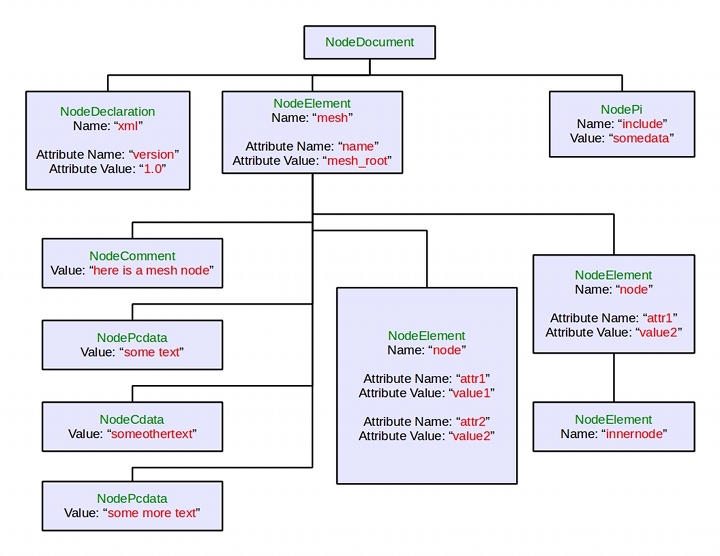
\includegraphics{SampleTree.jpg}
\caption{Complete Tree Representation of the Sample}
\end{DoxyImage}
  
\end{DoxyItemize}\hypertarget{XMLManual_XMLInterface}{}\subsubsection{C++ interface}\label{XMLManual_XMLInterface}
Despite the fact that there are several node types, there are only three C++ classes representing the tree (\hyperlink{classphys_1_1xml_1_1Document}{phys::xml::Document}, \hyperlink{classphys_1_1xml_1_1Node}{phys::xml::Node}, \hyperlink{classphys_1_1xml_1_1Attribute}{phys::xml::Attribute}); some operations on \hyperlink{classphys_1_1xml_1_1Node}{phys::xml::Node} are only valid for certain node types. The classes are described below. \par
 \par
 \hyperlink{classphys_1_1xml_1_1Document}{phys::xml::Document} is the owner of the entire document structure; it is a non-\/copyable class. The interface of \hyperlink{classphys_1_1xml_1_1Document}{phys::xml::Document} consists of loading functions ( see \hyperlink{XMLManual_XMLLoading}{Loading Documents} ), saving functions ( see \hyperlink{XMLManual_XMLSaving}{Saving Documents} ) and the entire interface of \hyperlink{classphys_1_1xml_1_1Node}{phys::xml::Node}, which allows for document inspection and/or modification. Note that while \hyperlink{classphys_1_1xml_1_1Document}{phys::xml::Document} is a sub-\/class of \hyperlink{classphys_1_1xml_1_1Node}{phys::xml::Node}, \hyperlink{classphys_1_1xml_1_1Node}{phys::xml::Node} is not a polymorphic type; the inheritance is present only to simplify usage. Alternatively you can use the \hyperlink{classphys_1_1xml_1_1Document_a93d8521e3241281e15f77cf7568d5754}{phys::xml::Document::DocumentElement} function to get the element node that's the immediate child of the document. \par
 \par
 Default constructor of \hyperlink{classphys_1_1xml_1_1Document}{phys::xml::Document} initializes the document to the tree with only a root node ( \hyperlink{classphys_1_1xml_1_1Document}{phys::xml::Document} node). You can then populate it with data using either tree modification functions or loading functions; all loading functions destroy the previous tree with all occupied memory, which puts existing node/attribute handles for this document to invalid state. If you want to destroy the previous tree, you can use the \hyperlink{classphys_1_1xml_1_1Document_a9ab556271e4a1214ecb35ba6aef9e8e4}{phys::xml::Document::Reset} function; it destroys the tree and replaces it with either an empty one or a copy of the specified document. Destructor of \hyperlink{classphys_1_1xml_1_1Document}{phys::xml::Document} also destroys the tree, thus the lifetime of the document object should exceed the lifetimes of any node/attribute handles that point to the tree. \begin{DoxyWarning}{Warning}
While technically node/attribute handles can be alive when the tree they're referring to is destroyed, calling any member function for these handles results in undefined behavior. Thus it is recommended to make sure that the document is destroyed only after all references to its nodes/attributes are destroyed.
\end{DoxyWarning}
\hyperlink{classphys_1_1xml_1_1Node}{phys::xml::Node} is the handle to a document node; it can point to any node in the document, including the document node itself. There is a common interface for nodes of all types; the actual node type can be queried via the \hyperlink{classphys_1_1xml_1_1Node_a33288f89218baf24d1061c6eeb08687f}{phys::xml::Node::Type()} method. Note that \hyperlink{classphys_1_1xml_1_1Node}{phys::xml::Node} is only a handle to the actual node, not the node itself -\/ you can have several phys::xml::node handles pointing to the same underlying object. Destroying \hyperlink{classphys_1_1xml_1_1Node}{phys::xml::Node} handle does not destroy the node and does not remove it from the tree. The size of \hyperlink{classphys_1_1xml_1_1Node}{phys::xml::Node} is equal to that of a pointer, so it is nothing more than a lightweight wrapper around a pointer; you can safely pass or return \hyperlink{namespacephys_1_1xml}{phys::xml}:Node objects by value without additional overhead. \par
 \par
 There is a special value of \hyperlink{classphys_1_1xml_1_1Node}{phys::xml::Node} type, known as null node or empty node (such nodes have type NodeNull). It does not correspond to any node in any document, and thus resembles null pointer. However, all operations are defined on empty nodes; generally the operations don't do anything and return empty nodes/attributes or empty strings as their result (see documentation for specific functions for more detailed information). This is useful for chaining calls; i.e. you can get the grandparent of a node like so: node.GetParent().GetParent(); if a node is a null node or it does not have a parent, the first Node::GetParent() call returns null node; the second GetParent() call then also returns null node, which can make error handling easier. \par
 \par
 \hyperlink{classphys_1_1xml_1_1Attribute}{phys::xml::Attribute} is a handle to an XML attribute; it has the same semantics as \hyperlink{classphys_1_1xml_1_1Node}{phys::xml::Node}, i.e. there can be several \hyperlink{classphys_1_1xml_1_1Attribute}{phys::xml::Attribute} handles pointing to the same underlying object and there is a special null attribute value, which propagates to function results. \par
 \par
 Both \hyperlink{classphys_1_1xml_1_1Node}{phys::xml::Node} and \hyperlink{classphys_1_1xml_1_1Attribute}{phys::xml::Attribute} have the default constructor which initializes them to null objects. \par
 \par
 \hyperlink{classphys_1_1xml_1_1Node}{phys::xml::Node} and \hyperlink{classphys_1_1xml_1_1Attribute}{phys::xml::Attribute} try to behave like pointers, that is, they can be compared with other objects of the same type, making it possible to use them as keys in associative containers. All handles to the same underlying object are equal, and any two handles to different underlying objects are not equal. Null handles only compare as equal to themselves. The result of relational comparison can not be reliably determined from the order of nodes in file or in any other way. Do not use relational comparison operators except for search optimization (i.e. associative container keys). \par
 \par
 If you want to use \hyperlink{classphys_1_1xml_1_1Node}{phys::xml::Node} or \hyperlink{classphys_1_1xml_1_1Attribute}{phys::xml::Attribute} objects as keys in hash-\/based associative containers, you can use the \hyperlink{classphys_1_1xml_1_1Node_a830a1833c4b4b012f1b4481e91ccb1ca}{phys::xml::Node::HashValue} or \hyperlink{classphys_1_1xml_1_1Attribute_ac0c27e07b705c41670a0903f4fe18378}{phys::xml::Attribute::HashValue} member functions. They return the hash values that are guaranteed to be the same for all handles to the same underlying object. The hash value for null handles is 0. \par
 \par
 Finally handles can be implicitly cast to boolean-\/like objects, so that you can test if the node/attribute is empty with the following code: if (node) \{ ... \} or if (!node) \{ ... \} else \{ ... \}. Alternatively you can check if a given Node/Attribute handle is null by calling the \hyperlink{classphys_1_1xml_1_1Attribute_a6d0157a562f283e9c87d1cc46b3405cc}{phys::xml::Attribute::Empty} or the \hyperlink{classphys_1_1xml_1_1Node_a22c00132e42702d16468489ff0bd01d8}{phys::xml::Node::Empty} Methods. \par
 \par
 Nodes and attributes do not exist without a document tree, so you can't create them without adding them to some document. Once underlying node/attribute objects are destroyed, the handles to those objects become invalid. While this means that destruction of the entire tree invalidates all node/attribute handles, it also means that destroying a subtree ( by calling \hyperlink{classphys_1_1xml_1_1Node_a946bb656b94c9d3a561200cd2cd3ee11}{phys::xml::Node::RemoveChild} ) or removing an attribute invalidates the corresponding handles. There is no way to check handle validity; you have to ensure correctness through external mechanisms. \par
 \par
 \hypertarget{XMLManual_XMLUnicode}{}\subsubsection{Unicode Interface}\label{XMLManual_XMLUnicode}
There are two choices of interface and internal representation when working with \hyperlink{namespacephys_1_1xml}{phys::xml} : you can either choose the UTF-\/8 (also called char) interface or UTF-\/16/32 (also called wchar\_\-t) one. The choice is controlled via XML\_\-WCHAR\_\-MODE define; you can set it via \hyperlink{xml_8h}{xml.h} or via preprocessor options beore engine compilation. If this define is set, the wchar\_\-t interface is used; otherwise (by default) the char interface is used. The exact wide character encoding is assumed to be either UTF-\/16 or UTF-\/32 and is determined based on the size of wchar\_\-t type. \begin{DoxyWarning}{Warning}
There are a few places that the reset of the engine assumes the use of the UTF-\/8/char interface. The task of integrating this cleanly is currently considered a low priority. If you use XML\_\-WCHAR\_\-MODE you will encounter bugs, they could be tiny or huge. Since we didn't test it, we assumed it doesn't work.
\end{DoxyWarning}
\begin{DoxyNote}{Note}
If the size of wchar\_\-t is 2, \hyperlink{namespacephys_1_1xml}{phys::xml} assumes UTF-\/16 encoding instead of UCS-\/2, which means that some characters are represented as two code points.
\end{DoxyNote}
All tree functions that work with strings work with either C-\/style null terminated strings or STL strings of the selected character type. For example, node name accessors look like this in char mode: 
\begin{DoxyCode}
 const char* phys::xml::Node::Name() const;
 bool phys::xml::Node::SetName(const char* value);
\end{DoxyCode}
 and like this in wchar\_\-t mode: 
\begin{DoxyCode}
 const wchar_t* phys::xml::Node::Name() const;
 bool phys::xml::Node::SetName(const wchar_t* value);
\end{DoxyCode}
 There is a special type, \hyperlink{namespacephys_1_1xml_afc87705cd1c2917d87b879715a2d8f6e}{phys::xml::char\_\-t}, that is defined as the character type and depends on the engine configuration; it will be also used in the documentation hereafter. There is also a type phys::xml::string\_\-t, which is defined as the STL string of the character type; it corresponds to std::string in char mode and to std::wstring in wchar\_\-t mode. \begin{DoxyNote}{Note}
This is one our list of items to integrate more tighlty. At some point \hyperlink{namespacephys_1_1xml_afc87705cd1c2917d87b879715a2d8f6e}{phys::xml::char\_\-t} will be replace by \hyperlink{namespacephys_a3098bae5b0a3cd16eec331f766cc562b}{phys::Character}, and phys::xml::string\_\-t will be replaced by \hyperlink{namespacephys_aa03900411993de7fbfec4789bc1d392e}{phys::String}. For now they remain Interoperable.
\end{DoxyNote}
In addition to the interface, the internal implementation changes to store XML data as \hyperlink{namespacephys_1_1xml_afc87705cd1c2917d87b879715a2d8f6e}{phys::xml::char\_\-t}; this means that these two modes have different memory usage characteristics. The conversion to \hyperlink{namespacephys_1_1xml_afc87705cd1c2917d87b879715a2d8f6e}{phys::xml::char\_\-t} upon document loading and from \hyperlink{namespacephys_1_1xml_afc87705cd1c2917d87b879715a2d8f6e}{phys::xml::char\_\-t} upon document saving happen automatically, which also carries minor performance penalty. The general advice however is to select the character mode based on usage scenario, i.e. if UTF-\/8 is inconvenient to process and most of your XML data is non-\/ASCII, wchar\_\-t mode is probably a better choice (if this is the case any patches, notifications or bugfixes that could be sent our way would help.) \par
 \par
 There are cases when you'll have to convert string data between UTF-\/8 and wchar\_\-t encodings; the following helper functions are provided for such purposes: 
\begin{DoxyCode}
 std::string AsUtf8(const wchar_t* str);
 std::wstring AsUtf8(const char* str);
\end{DoxyCode}
 Both functions accept a null-\/terminated string as an argument str, and return the converted string. AsUtf8 performs conversion from UTF-\/16/32 to UTF-\/8; AsWide performs conversion from UTF-\/8 to UTF-\/16/32. Invalid UTF sequences are silently discarded upon conversion. str has to be a valid string; passing null pointer results in undefined behavior. There are also two overloads with the same semantics which accept a string as an argument: 
\begin{DoxyCode}
 std::string AsUtf8(const std::wstring& str);
 std::wstring AsWide(const std::string& str);
\end{DoxyCode}
 \begin{DoxyNote}{Note}
Most examples in this documentation assume char interface and therefore will not compile with XML\_\-WCHAR\_\-MODE. This is done to simplify the documentation; usually the only changes you'll have to make is to pass wchar\_\-t string literals, i.e. instead of \par
 \par
 
\begin{DoxyCode}
 phys::xml::Node node = doc.GetChild("bookstore").FindChildbyAttribute("book", "i
      d", "12345"); 
\end{DoxyCode}
 \par
 \par
 you'll have to do \par
 \par
 
\begin{DoxyCode}
 phys::xml::Node node = doc.GetChild(L"bookstore").FindChildbyAttribute(L"book", 
      L"id", L"12345"); 
\end{DoxyCode}

\end{DoxyNote}
\hypertarget{XMLManual_XMLThreadSafety}{}\subsubsection{Thread-\/safety guarantees}\label{XMLManual_XMLThreadSafety}
Almost all functions in \hyperlink{namespacephys_1_1xml}{phys::xml} have the following thread-\/safety guarantees:
\begin{DoxyItemize}
\item It is safe to call free (non-\/member) functions from multiple threads
\item It is safe to perform concurrent read-\/only accesses to the same tree (all constant member functions do not modify the tree)
\item It is safe to perform concurrent read/write accesses, if there is only one read or write access to the single tree at a time
\end{DoxyItemize}

Concurrent modification and traversing of a single tree requires synchronization, for example via reader-\/writer lock. Modification includes altering document structure and altering individual node/attribute data, i.e. changing names/values. \par
 \par
 The only exception is phys::SetMemory\_\-management\_\-functions; it modifies global variables and as such is not thread-\/safe. Its usage policy has more restrictions, see \hyperlink{XMLManual_XMLCustomAlloc}{Custom memory allocation/deallocation functions} . \hypertarget{XMLManual_XMLExceptionSafety}{}\subsubsection{Exception guarantees}\label{XMLManual_XMLExceptionSafety}
With the exception of XPath, \hyperlink{namespacephys_1_1xml}{phys::xml} itself does not throw any exceptions. Additionally, most \hyperlink{namespacephys_1_1xml}{phys::xml} functions have a no-\/throw exception guarantee. \par
 \par
 This is not applicable to functions that operate on STL strings or IOstreams; such functions have either strong guarantee (functions that operate on strings) or basic guarantee (functions that operate on streams). Also functions that call user-\/defined callbacks (i.e. \hyperlink{classphys_1_1xml_1_1Node_a0029d08d3689c36d882ada0c0c9cf6e9}{phys::xml::Node::Traverse} or \hyperlink{classphys_1_1xml_1_1Node_ab2311cefdf1d7f4886cbebd7350d7731}{phys::xml::Node::FindNode}) do not provide any exception guarantees beyond the ones provided by the callback. \par
 \par
 If exception handling is not disabled with XML\_\-NO\_\-EXCEPTIONS define, XPath functions may throw \hyperlink{classphys_1_1xml_1_1XPathException}{phys::xml::XPathException} on parsing errors; also, XPath functions may throw std::bad\_\-alloc in low memory conditions. Still, XPath functions provide strong exception guarantee. \hypertarget{XMLManual_XMLMemory}{}\subsubsection{Memory management}\label{XMLManual_XMLMemory}
Still in progress \hypertarget{XMLManual_XMLCustomAlloc}{}\paragraph{Custom memory allocation/deallocation functions}\label{XMLManual_XMLCustomAlloc}
Still in progress \hypertarget{XMLManual_XMLMemoryInternals}{}\paragraph{Document memory management internals}\label{XMLManual_XMLMemoryInternals}
Still in progress \hypertarget{XMLManual_XMLUnicode}{}\subsubsection{Unicode Interface}\label{XMLManual_XMLUnicode}
Still in progress \hypertarget{XMLManual_XMLLoading}{}\subsection{Loading Documents}\label{XMLManual_XMLLoading}
Still in progress \hypertarget{XMLManual_XMLAccessing}{}\subsection{Accessing Document Data}\label{XMLManual_XMLAccessing}
Still in progress \hypertarget{XMLManual_XMLModifying}{}\subsection{Modifiying Document}\label{XMLManual_XMLModifying}
Still in progress \hypertarget{XMLManual_XMLSaving}{}\subsection{Saving Documents}\label{XMLManual_XMLSaving}
Still in progress \hypertarget{XMLManual_XMLXPath}{}\subsection{XMLXPath}\label{XMLManual_XMLXPath}
Still in progress 